\section{Проблема}

Современные фреймворки предоставляют два основных способа задания графов: композиция примитивных операций (\textit{Map}, \textit{Reduce} и т.д.) и SQL запросы (диалект Streaming SQL, для потоковой обработки \cite{streaming-sql}). На рисунке \ref{fig:api-stack} представлена иерархия  Apache Flink API.

\begin{figure}[h]
    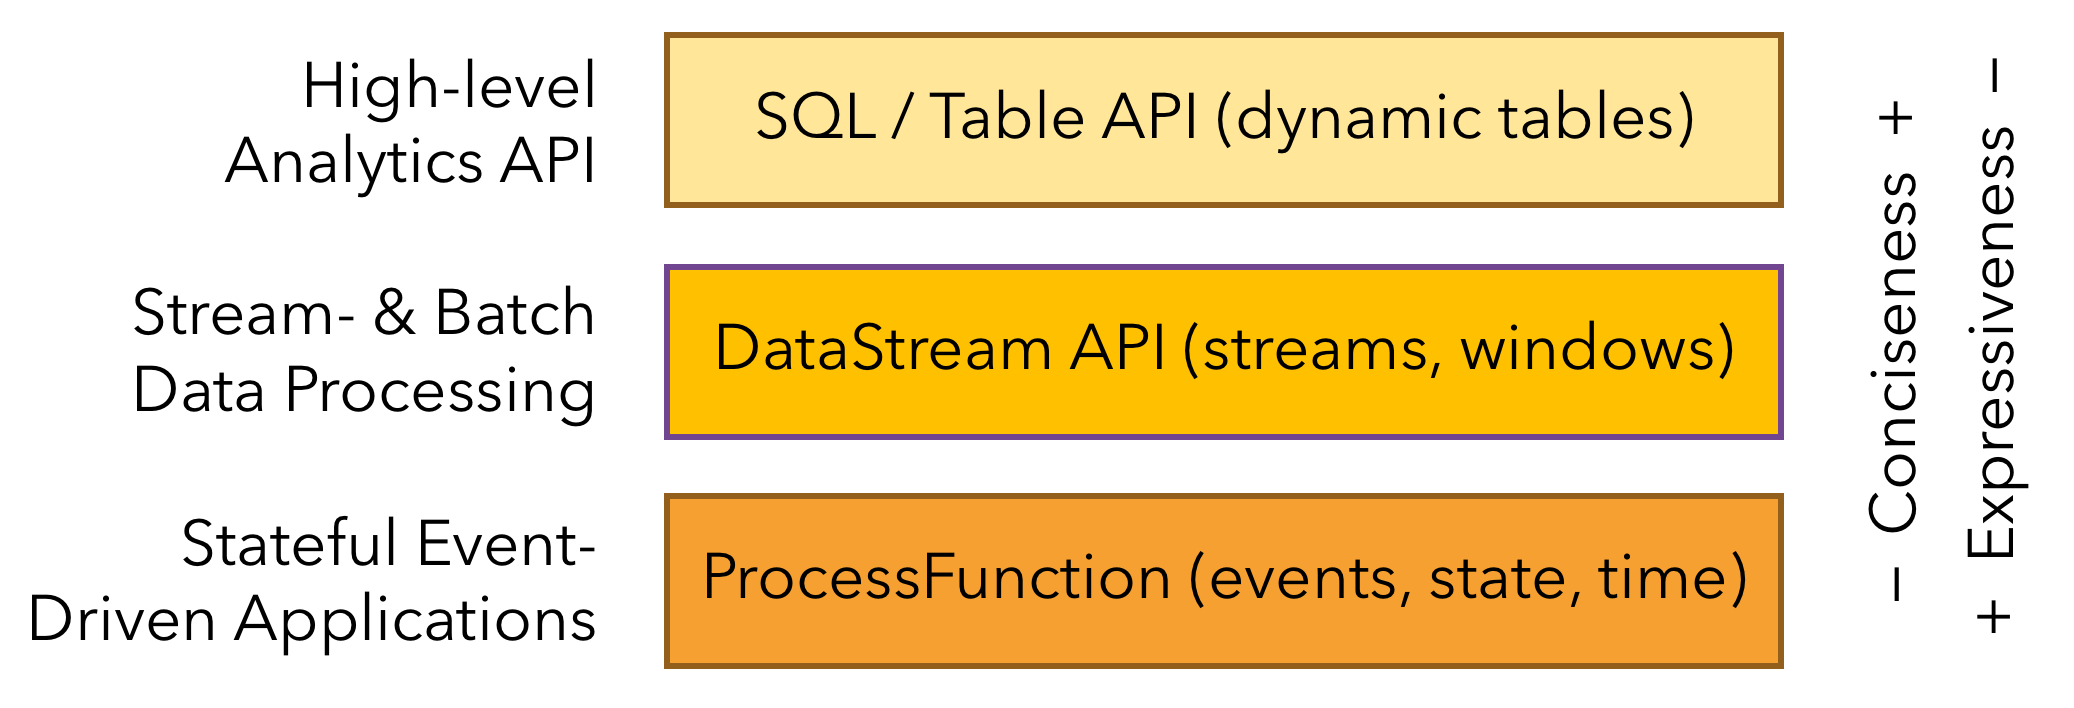
\includegraphics[width=\linewidth]{api-stack.png}
    \caption{Иерархия Apache Flink API. Видим, что фреймворк предоставляет три уровня интерфейсов: от самого выразительного, \textit{ProcessFunction}, до самого лаконичного, SQL. \textit{ProcessFunction} и \textit{DataStream} позволяют определять операции и составлять их композиции.}
    \label{fig:api-stack}
\end{figure}

Пусть мы хотим записать граф, схематично изображенный на рисунке \ref{fig:complex-graph}.

\begin{figure}[h]
    \centering
    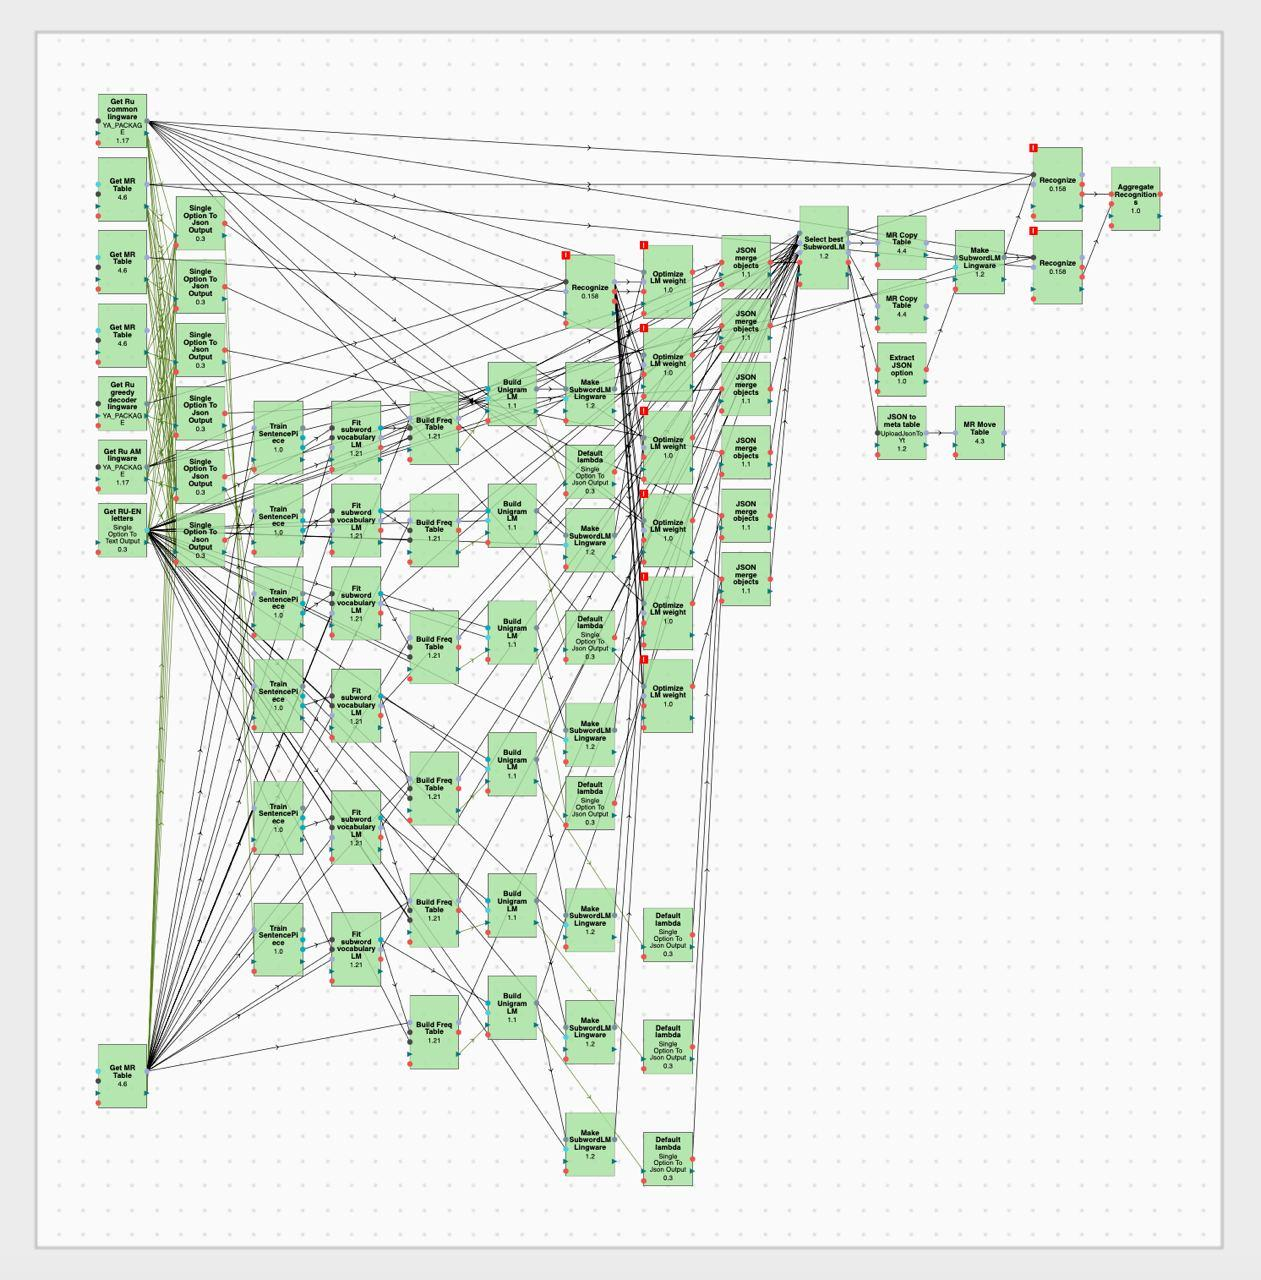
\includegraphics[width=0.8\linewidth]{complex-graph.jpg}
    \caption{Графы, производящие обработку данных для реальных приложений могут быть довольно большими.}
    \label{fig:complex-graph}
\end{figure}

Когда мы составляем граф как композицию операций (как на рисунке \ref{fig:prog-data}),
мы однозначно определяем их порядок и не предоставляем фреймворку информации о том,
какие операции с какими можно переставлять в целях оптимизации, оставляя пайплайн корректным.
Таким образом, возможна только ручная оптимизация.

Диалект Streaming SQL позволяет использовать в SQL запросах неограниченные источники данных.
Как и в случае с традиционным SQL, он предназначен для выборки данных из источников и подсчёта статистик, а не для записи комплексной бизнес-логики.

Пусть мы уже имеем написанный и работающий на кластере граф \ref{fig:complex-graph}.
Попробуем добавить этому графу ещё одну функциональность и вернуть на кластер.
Постараемся максимально использовать промежуточные значения, вычисленные в исходном графе, чтобы не производить лишних повторных вычислений.

Сейчас для таких модификаций требуется вручную исправлять граф и производить оптимизации (минимизировать количество решардирований, размещать фильтрации как можно ближе к источникам данных и т.д.). В случае больших графов это довольно сложная работа, подверженная трудно уловимым ошибкам.

Таким образом, требуется разработать декларативный подход к описанию вычислительных графов, который бы упростил их задание и модификацию, и позволил бы производить автоматические оптимизации путём перестановки операций в графе.
